\section{Reactor Models}
\label{sec:reactor_models}

In this work, we will explore various transition scenarios for the deployment in the \gls{usa} of the: 1) \gls{xe}-like \glspl{htgr}; 2) \gls{usnc} \gls{mmr}-like \glspl{htgr}; and 3) and Westinghouse AP1000-like \glspl{pwr}. To accommodate our assumption that the \gls{haleu} fueled \gls{triso} reactors will first accept \gls{leup} fuel, we have adapted Bachmann's \gls{mmr}-like Serpent model \cite{bachmann_mmr_like_2023} and Richter's \gls{xe}-like Serpent model \cite{richter_xe100_like} to accept \gls{leup} fuel. These reactor models are not based on confidential or proprietary information, they are constructed from publicly available data to approximate the aggregate behavior.

\begin{table}[!htbp]
   \centering
   \caption{Advanced reactor design specifications.}
   \label{tab:ar_defs}
   \begin{tabular}{c c c c}
      \hline
      \textbf{Design Criteria} & \textbf{MMR-Like} \cite{usnc_design_2021} & \textbf{\gls{xe}-Like} \cite{nuscale_chapter_2018} & \textbf{AP1000} \\
      \hline
      Reactor type & \gls{htgr} & \gls{htgr} & \gls{pwr} \\
      Power Output [MWth] & 15 & 100 & 1000 \\
      Fuel Type & \gls{triso} & \gls{triso} & UO$_2$ \\
      Enrichment [\% $^{235}$U] & 9.95, 19.75 & 9.95, 15.5 & 5 \\
      Cycle Length [yrs] & 20 & Online Refuel & 18 \\
      Discharge Burnup [GWd/MTU] & 82 & 168 & 65 \\
      Reactor Lifetime [yrs] & 20 & 60 & 60 \\
      \hline
   \end{tabular}
\end{table}

In the following subsections, we will discuss the reactors in greater detail. One limitation of this work that we will devote future research to is the approximation for the \gls{leup} fueled version of the reactors as achieving the same burnup and power level as the \gls{haleu} fueled version. This assumption is not necessarily valid, and we will explore the implications of this assumption in future work. However, we expect that, due to the limited deployment of \gls{leup} fuel, the discrepancies will be well-understood.

\subsection{MMR-like Reactor}
\label{sec:mmr}

The future of the once-active partnership between \gls{uiuc} and \gls{usnc} to deploy their \gls{mmr} is uncertain to those not on the project; however, they reached the pre-licensing phase with the \gls{nrc} and were planning on commencing operation in the 2030s. The \gls{usnc} \gls{mmr} is a \gls{htgr} that uses \gls{triso} fuel. The reactor has a thermal output of 15 MW and a cycle length of 20 years. The fuel is enriched to 9.95\% $^{235}$U and has a discharge burnup of 82 GWd/MTU. The reactor has a lifetime of 20 years. The reactor in this work is an approximation based on publicly available data and is not based on confidential or proprietary information. The model was originally developed by Bachmann et al. \cite{bachmann_mmr_like_2023}, and is implemented in this work as-is for the \gls{haleu} version of the reactor while the \gls{leup} version is adapted from the \gls{haleu} version.

Figure \ref{fig:mmr_design} shows an artist's rendering of the \gls{mmr} core and reactor vessel. As indicated by the figure, the design is intended to be underground and they claim that the total reactor footprint will be less than 5 acres. The primary coolant is helium gas, which heats up in the core and deposits its heat in a heat exchanger to generate electricity to the side of the reactor \cite{usnc_chalk_river}. Helium is transparent to many nuclear interactions and is inert, making it an attractive choice for a coolant.

\begin{figure}[!htbp]
    \centering
    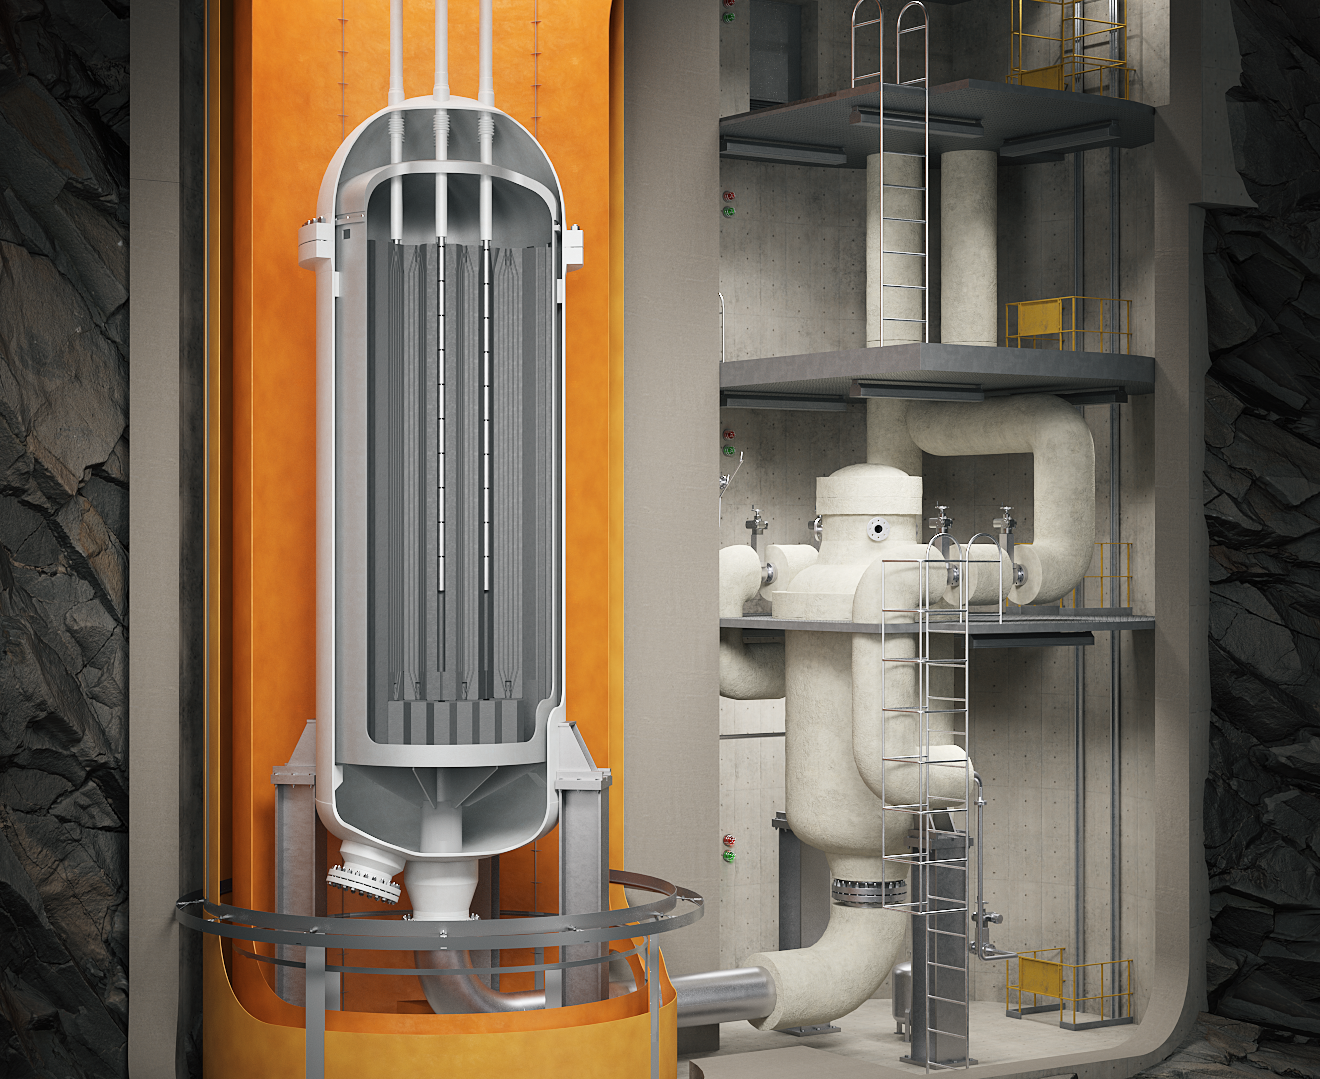
\includegraphics[scale=0.19]{images/reactor_design/wide-02.png}
    \caption{USNC MMR Design \cite{usnc_design_2021}}
    \label{fig:mmr_design}
\end{figure}

The company intends for an operational, what they call, "\gls{mmr} Energy System" to consist of two plants: the Nuclear Plant and the Adjacent Plant. The Nuclear Plant contains the multiple \gls{mmr} units including all the equipment required to transport the heat to the Adjacent Plant. The Adjacent Plant contains the equipment that converts heat to electricity or process heat as required. The \gls{mmr} Energy System will typically store up to 10 hours of power plant thermal output and can be supplemented with hydrogen burners. The use of molten salt thermal storage allows for flexibility in the supply of both electricity and process heat.

While the \gls{mmr} unit operates at constant power, electricity and heat are delivered on-demand from the power plant. The \gls{mmr}'s high temperature heat has many uses beyond generation of electricity. District heating, desalination, and process heat are all possible, and these use cases highlight the broader point that this generation of nuclear reactors are not solely intended for electricity generation as with the current \gls{usa} fleet. An \gls{mmr} could deliver steam temperatures of 660 °C, and they claim on their website that temperatures up 950 °C could be possible in future \gls{mmr} variants.

The fuel for this reactor is inspired by the \gls{triso} fuel developed in the 1960s and 1970s. The fuel is a small sphere of uranium fuel that is coated in layers of carbon and silicon carbide. As shown in Figure \ref{fig:usnc_fuel}, the fuel is composed of kernels arranged into a larger fuel pellet. They call their fuel form \gls{fcm} fuel. They additively manufacture each element, allowing for a high packing fraction of fuel and means their fuel could be adapted to many reactor designs.

\begin{figure}[!ht]
    \subfloat[Fuel element layers\label{fig:elemenet_layers}]{%
      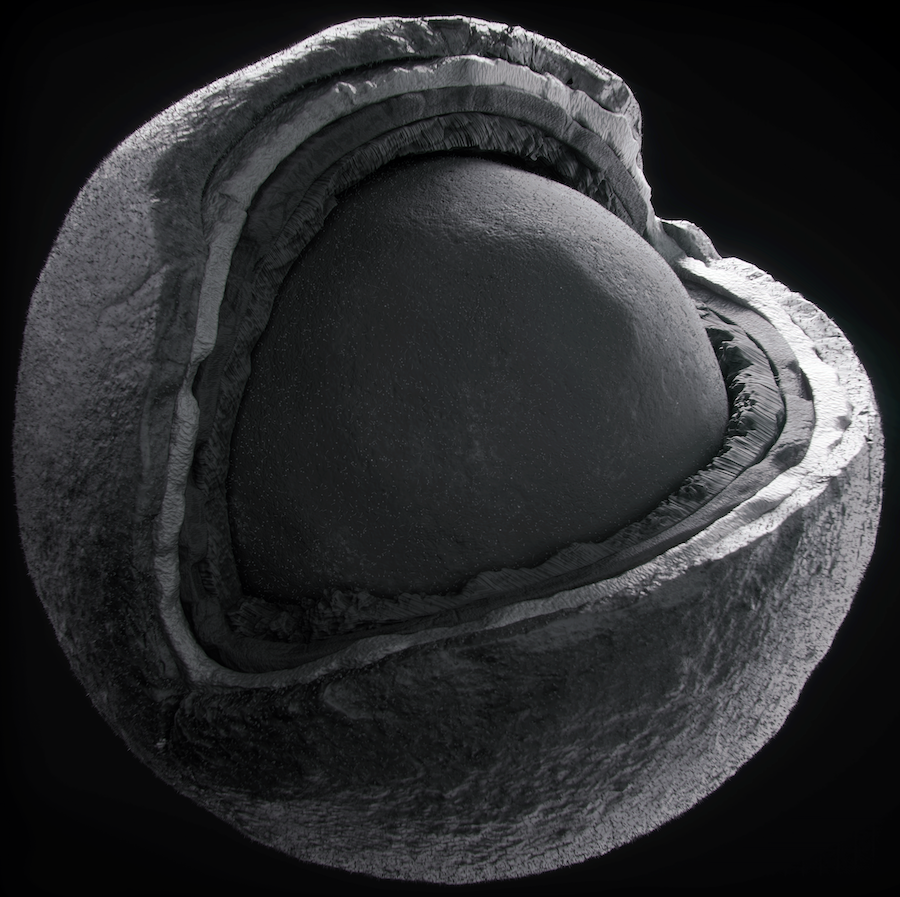
\includegraphics[width=0.49\textwidth]{images/reactor_design/usnc_triso.png}
   }
    \hfill
    \subfloat[Fuel pellet profile\label{fig:pellet_profile}]{%
      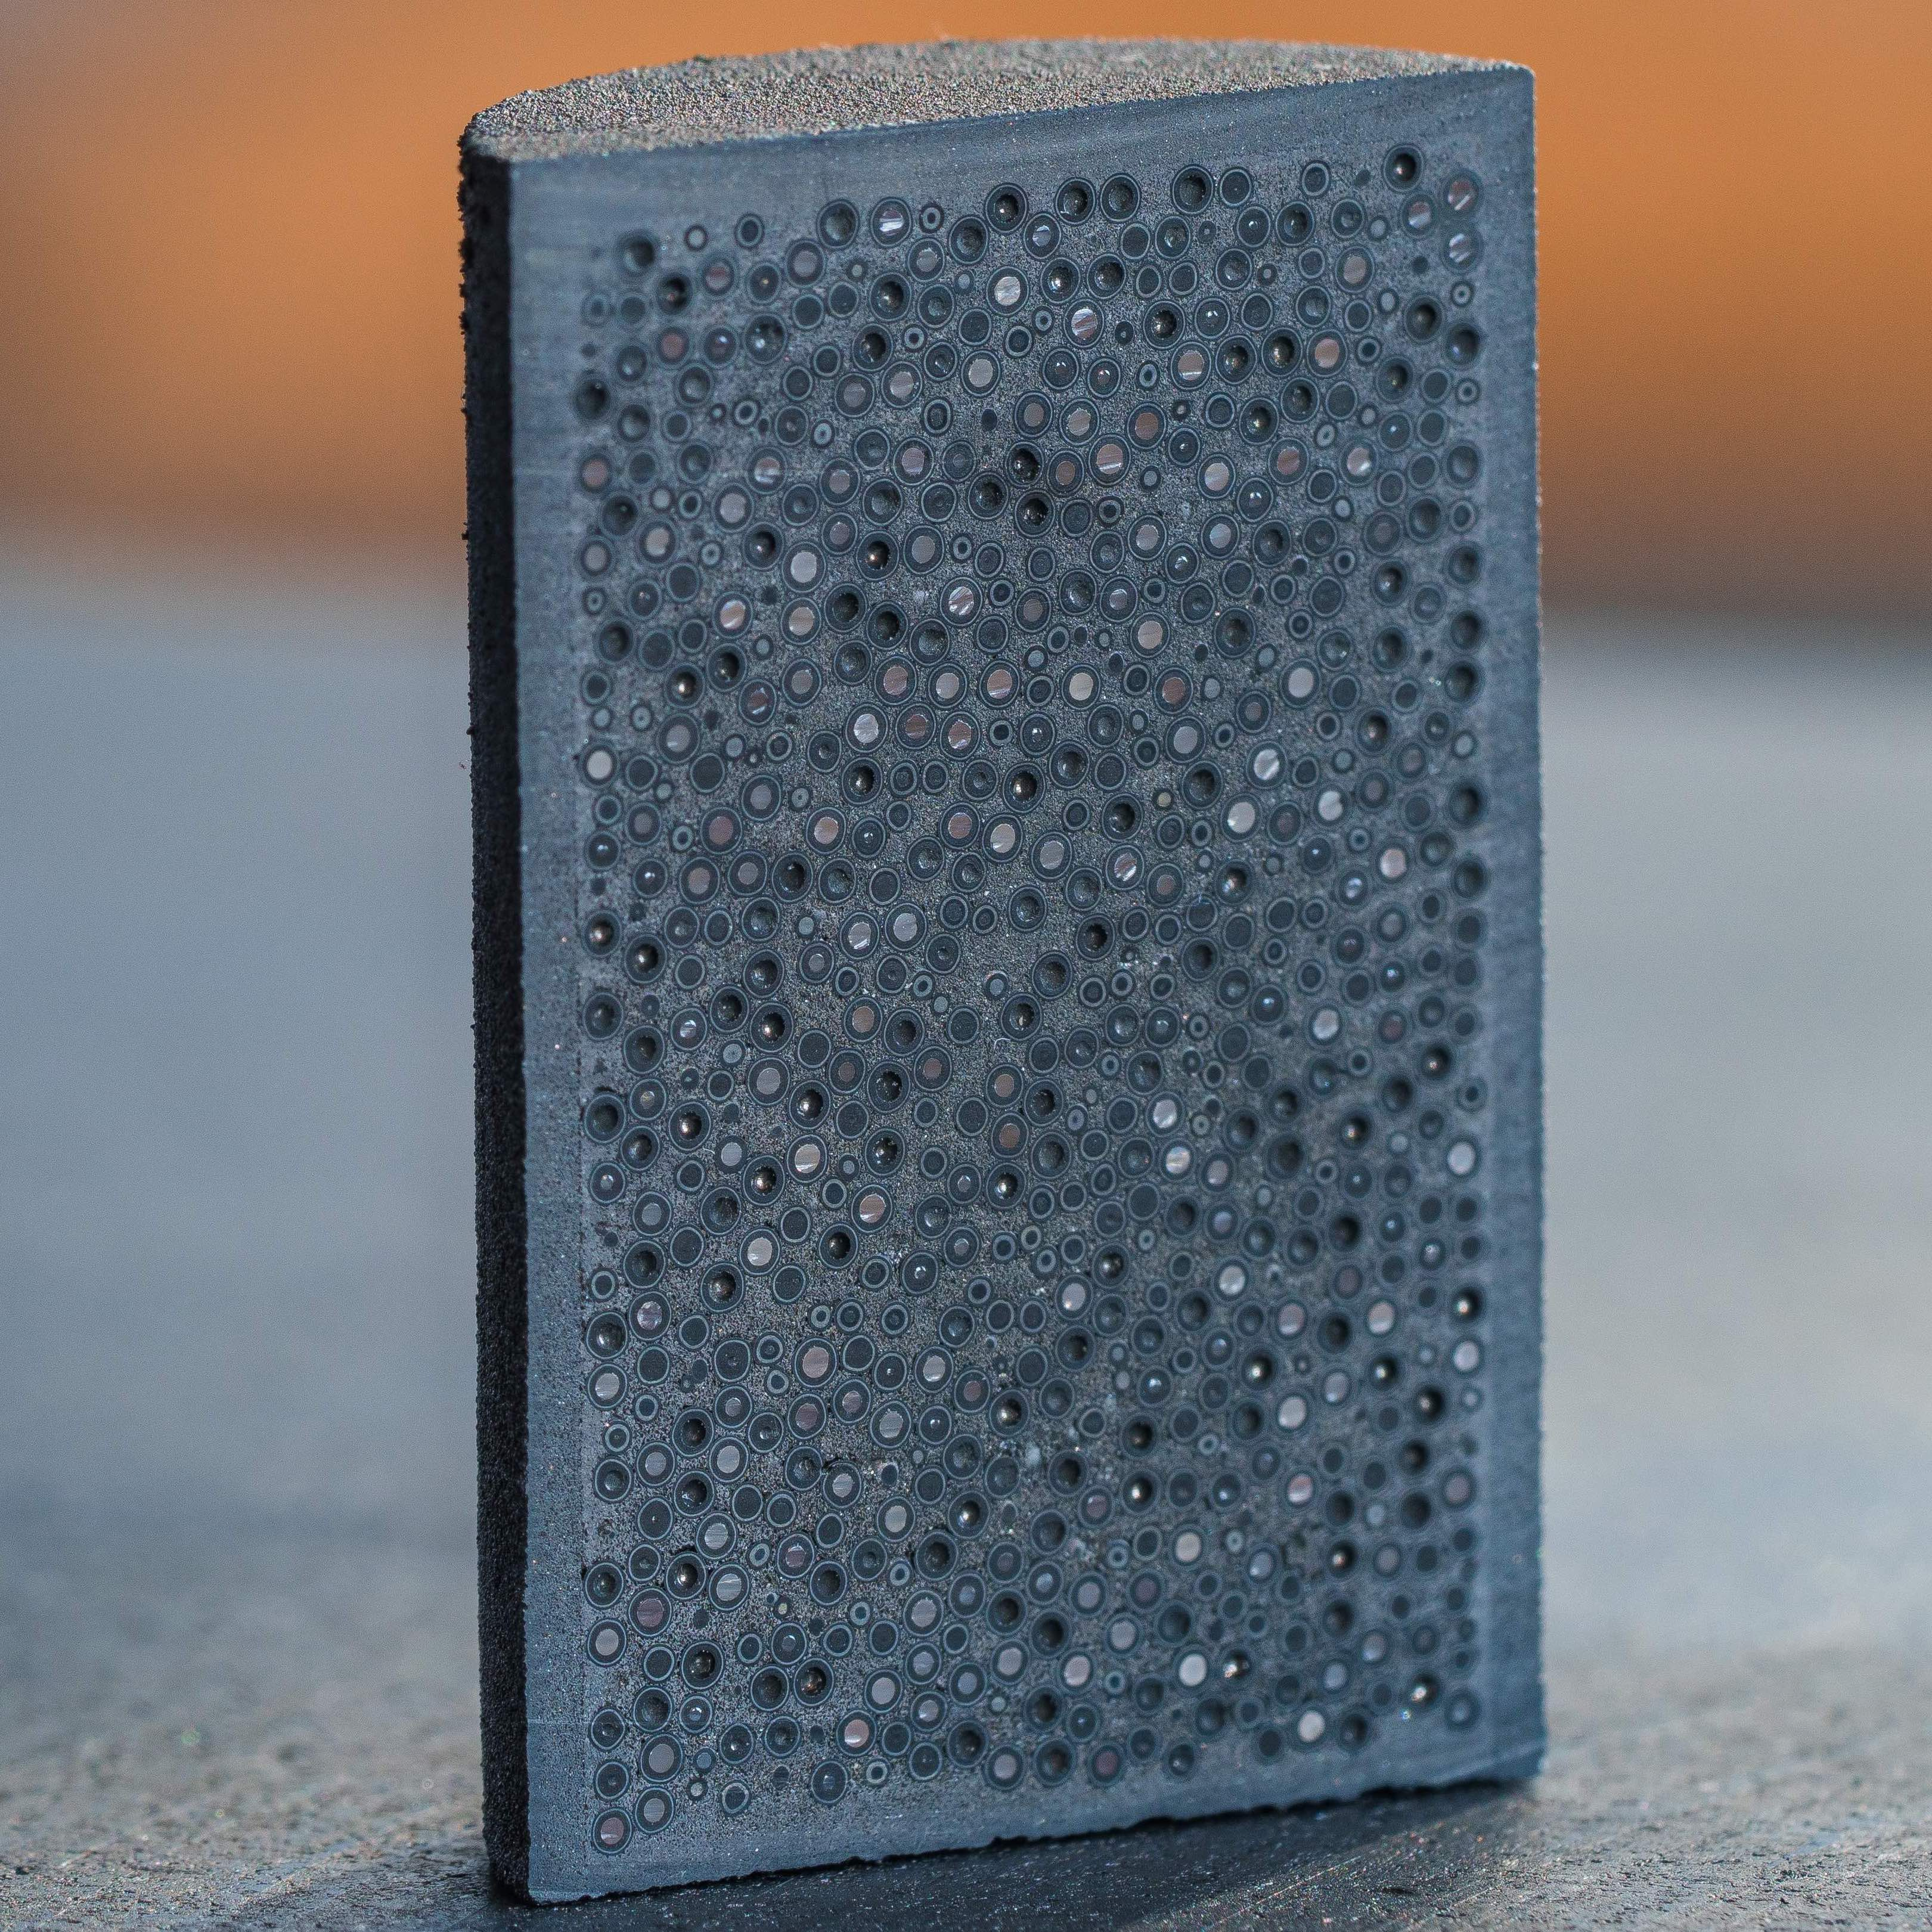
\includegraphics[width=0.49\textwidth]{images/reactor_design/usnc_fuel_side.jpeg}
   }
    \caption{
    USNC \gls{mmr} fuel renderings
      \cite{usnc_media_kit}}
    \label{fig:usnc_fuel}
\end{figure}

We have modified the fuel composition of Bachmann's \gls{mmr}-like reactor model to accept \gls{leup} fuel. The \gls{leup} fuel is assumed to have the same burnup and power level as the \gls{haleu} fuel. This assumption is not necessarily valid, and we will explore the implications of this assumption in future work; however, we expect that, due to the limited deployment of \gls{leup} fuel, the discrepancies will be well-understood. Figure \ref{fig:mmr_core} shows the top-down view of the \gls{mmr} core model, we will not display both the \gls{leup} and \gls{haleu} versions of the core as they are established by Bachmann \cite{bachmann_thesis_2023}.


\begin{figure}[!ht]
    \subfloat[Fuel element layers\label{fig:mmr_td}]{%
      
\includegraphics[width=0.49\textwidth]{images/reactor_design/haleu_mmr_2blocks.inp_geom1.png}
   }
    \hfill
    \subfloat[Fuel pellet profile\label{fig:mmr_slice}]{%
      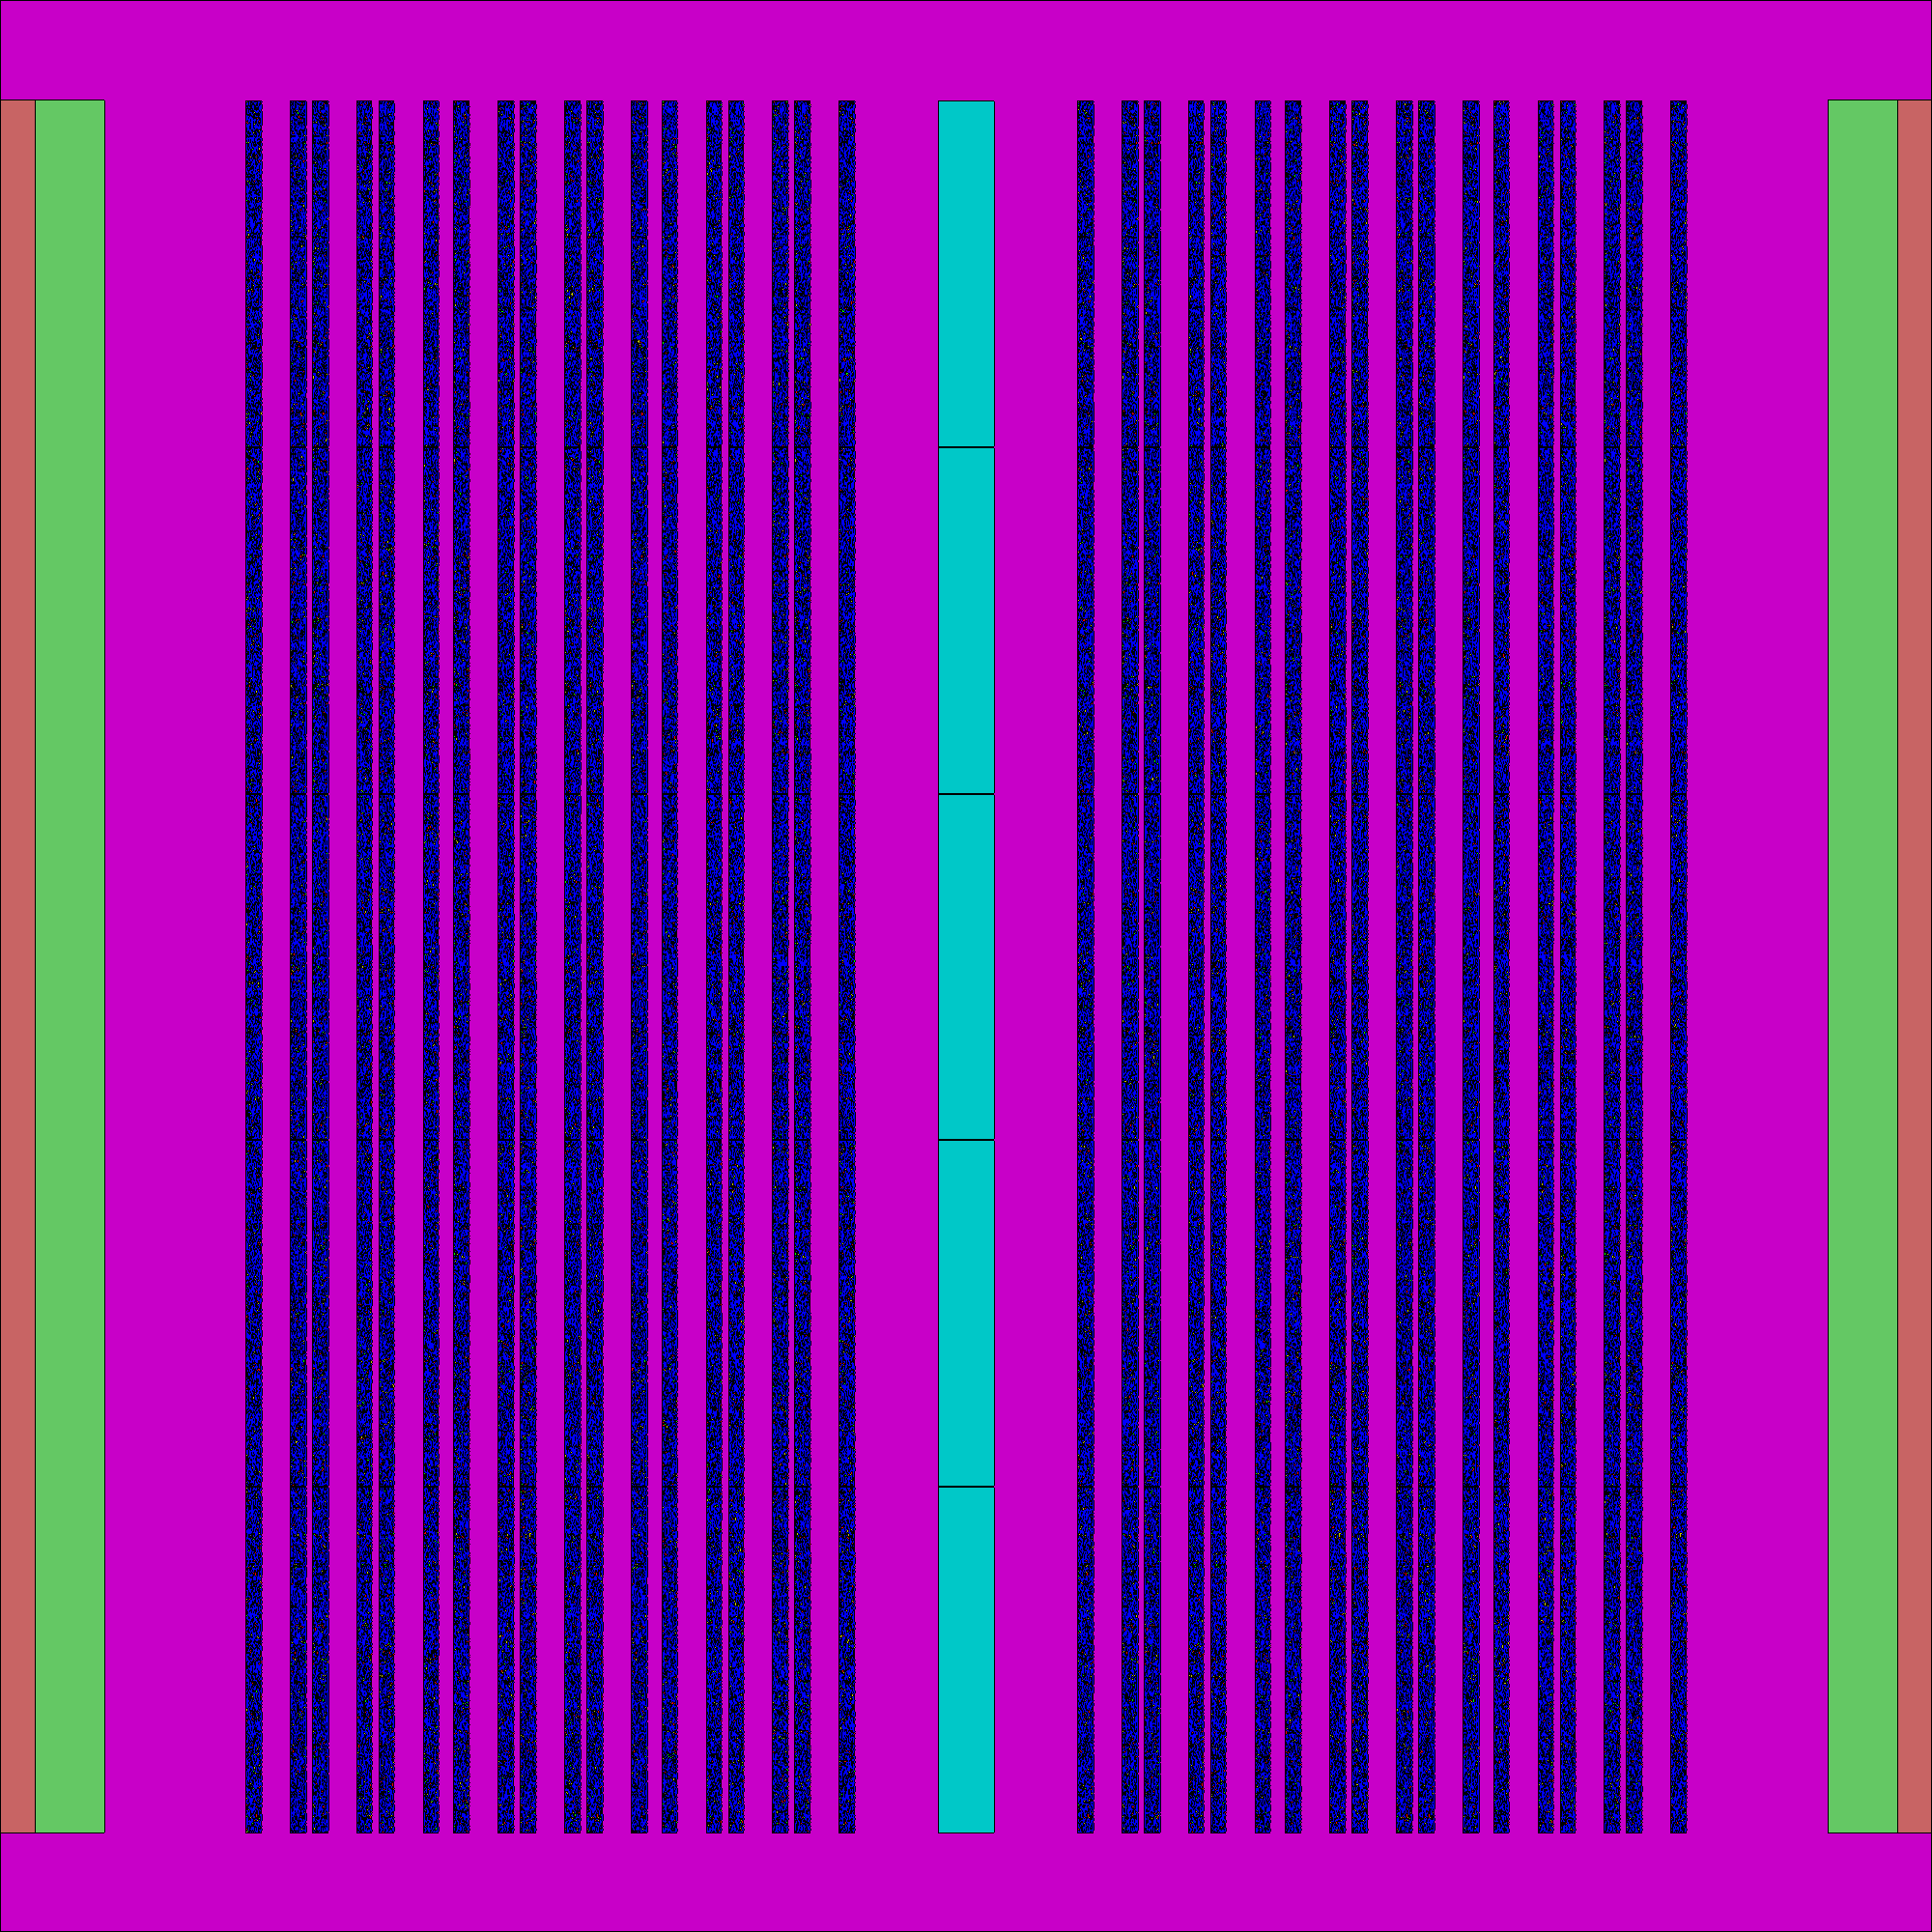
\includegraphics[width=0.49\textwidth]{images/reactor_design/haleu_mmr_2blocks.inp_geom3.png}
   }
    \caption{Serpent model of the USNC MMR core.}
    \label{fig:mmr_core}
\end{figure}

Figure \ref{fig:mmr_core} shows a top down and side view of the \gls{mmr} Serpent model \cite{bachmann_mmr_like_2023} that we have modified in fuel composition alone. As Bachmann describes \cite{bachmann_thesis_2023}, the radius of the fuel channel is based on the publicly available size of the \gls{fcm} pellets (1.15 cm) and the coolant channel has an arbitrarily chosen radius of 3 cm. The entire core is assumed to be in an isothermal state at 800 K. There is a 20 cm thick graphite reflector above and below the stacks of graphite, and a 10 cm thick beryllium-oxide reflector on the outside of the graphite blocks of the core, illustrated by the green material in Figure \ref{fig:mmr_core}. The control rods and burnable poisons are not included in this model, so the control rod locations are filled with helium. There are five layers of the graphite fuel blocks stacked to form the entire core, to approximate the number of fuel blocks described in \cite{usnc_design_2021}. The fuel does not move through the core, as the model is designed to use the same fuel for the entire lifetime of the reactor.



\subsection{\gls{xe}-like Reactor}
\label{sec:xe}

As of this writing, X-Energy has received a grant from the \gls{doe} to deploy their \gls{xe} in the pre-licensing phase with the \gls{nrc} for projects in Texas and Washington and is expected to be operational in the 2030s. There are similar projects in early stages in Canada and the \gls{uk}. The X-Energy \gls{xe} is a \gls{htgr} that uses \gls{triso} fuel. The reactor has a thermal output of 100 MW and uses online refueling. The fuel is enriched to 9.95\% $^{235}$U and has a discharge burnup of 168 GWd/MTU. The reactor has a lifetime of 60 years. The reactor in this work is an approximation based on publicly available data and is not based on confidential or proprietary information. The model was originally developed by Richter et al. \cite{richter_xe100_like}, and is implemented in this work as-is for the \gls{haleu} version of the reactor while the \gls{leup} version is adapted from the \gls{haleu} version.

Figure \ref{fig:xe_design} shows an artist's rendering of the \gls{xe} core and reactor vessel. The \gls{xe} reactor is designed to be a small modular reactor that can be deployed in a variety of locations, and is similar to the \gls{mmr} in that it is designed to be gas cooled. Where this design differs from the \gls{mmr} is that the reactor is designed to be refueled online, due to its pebble-bed nature.

\begin{figure}[!htbp]
    \centering
    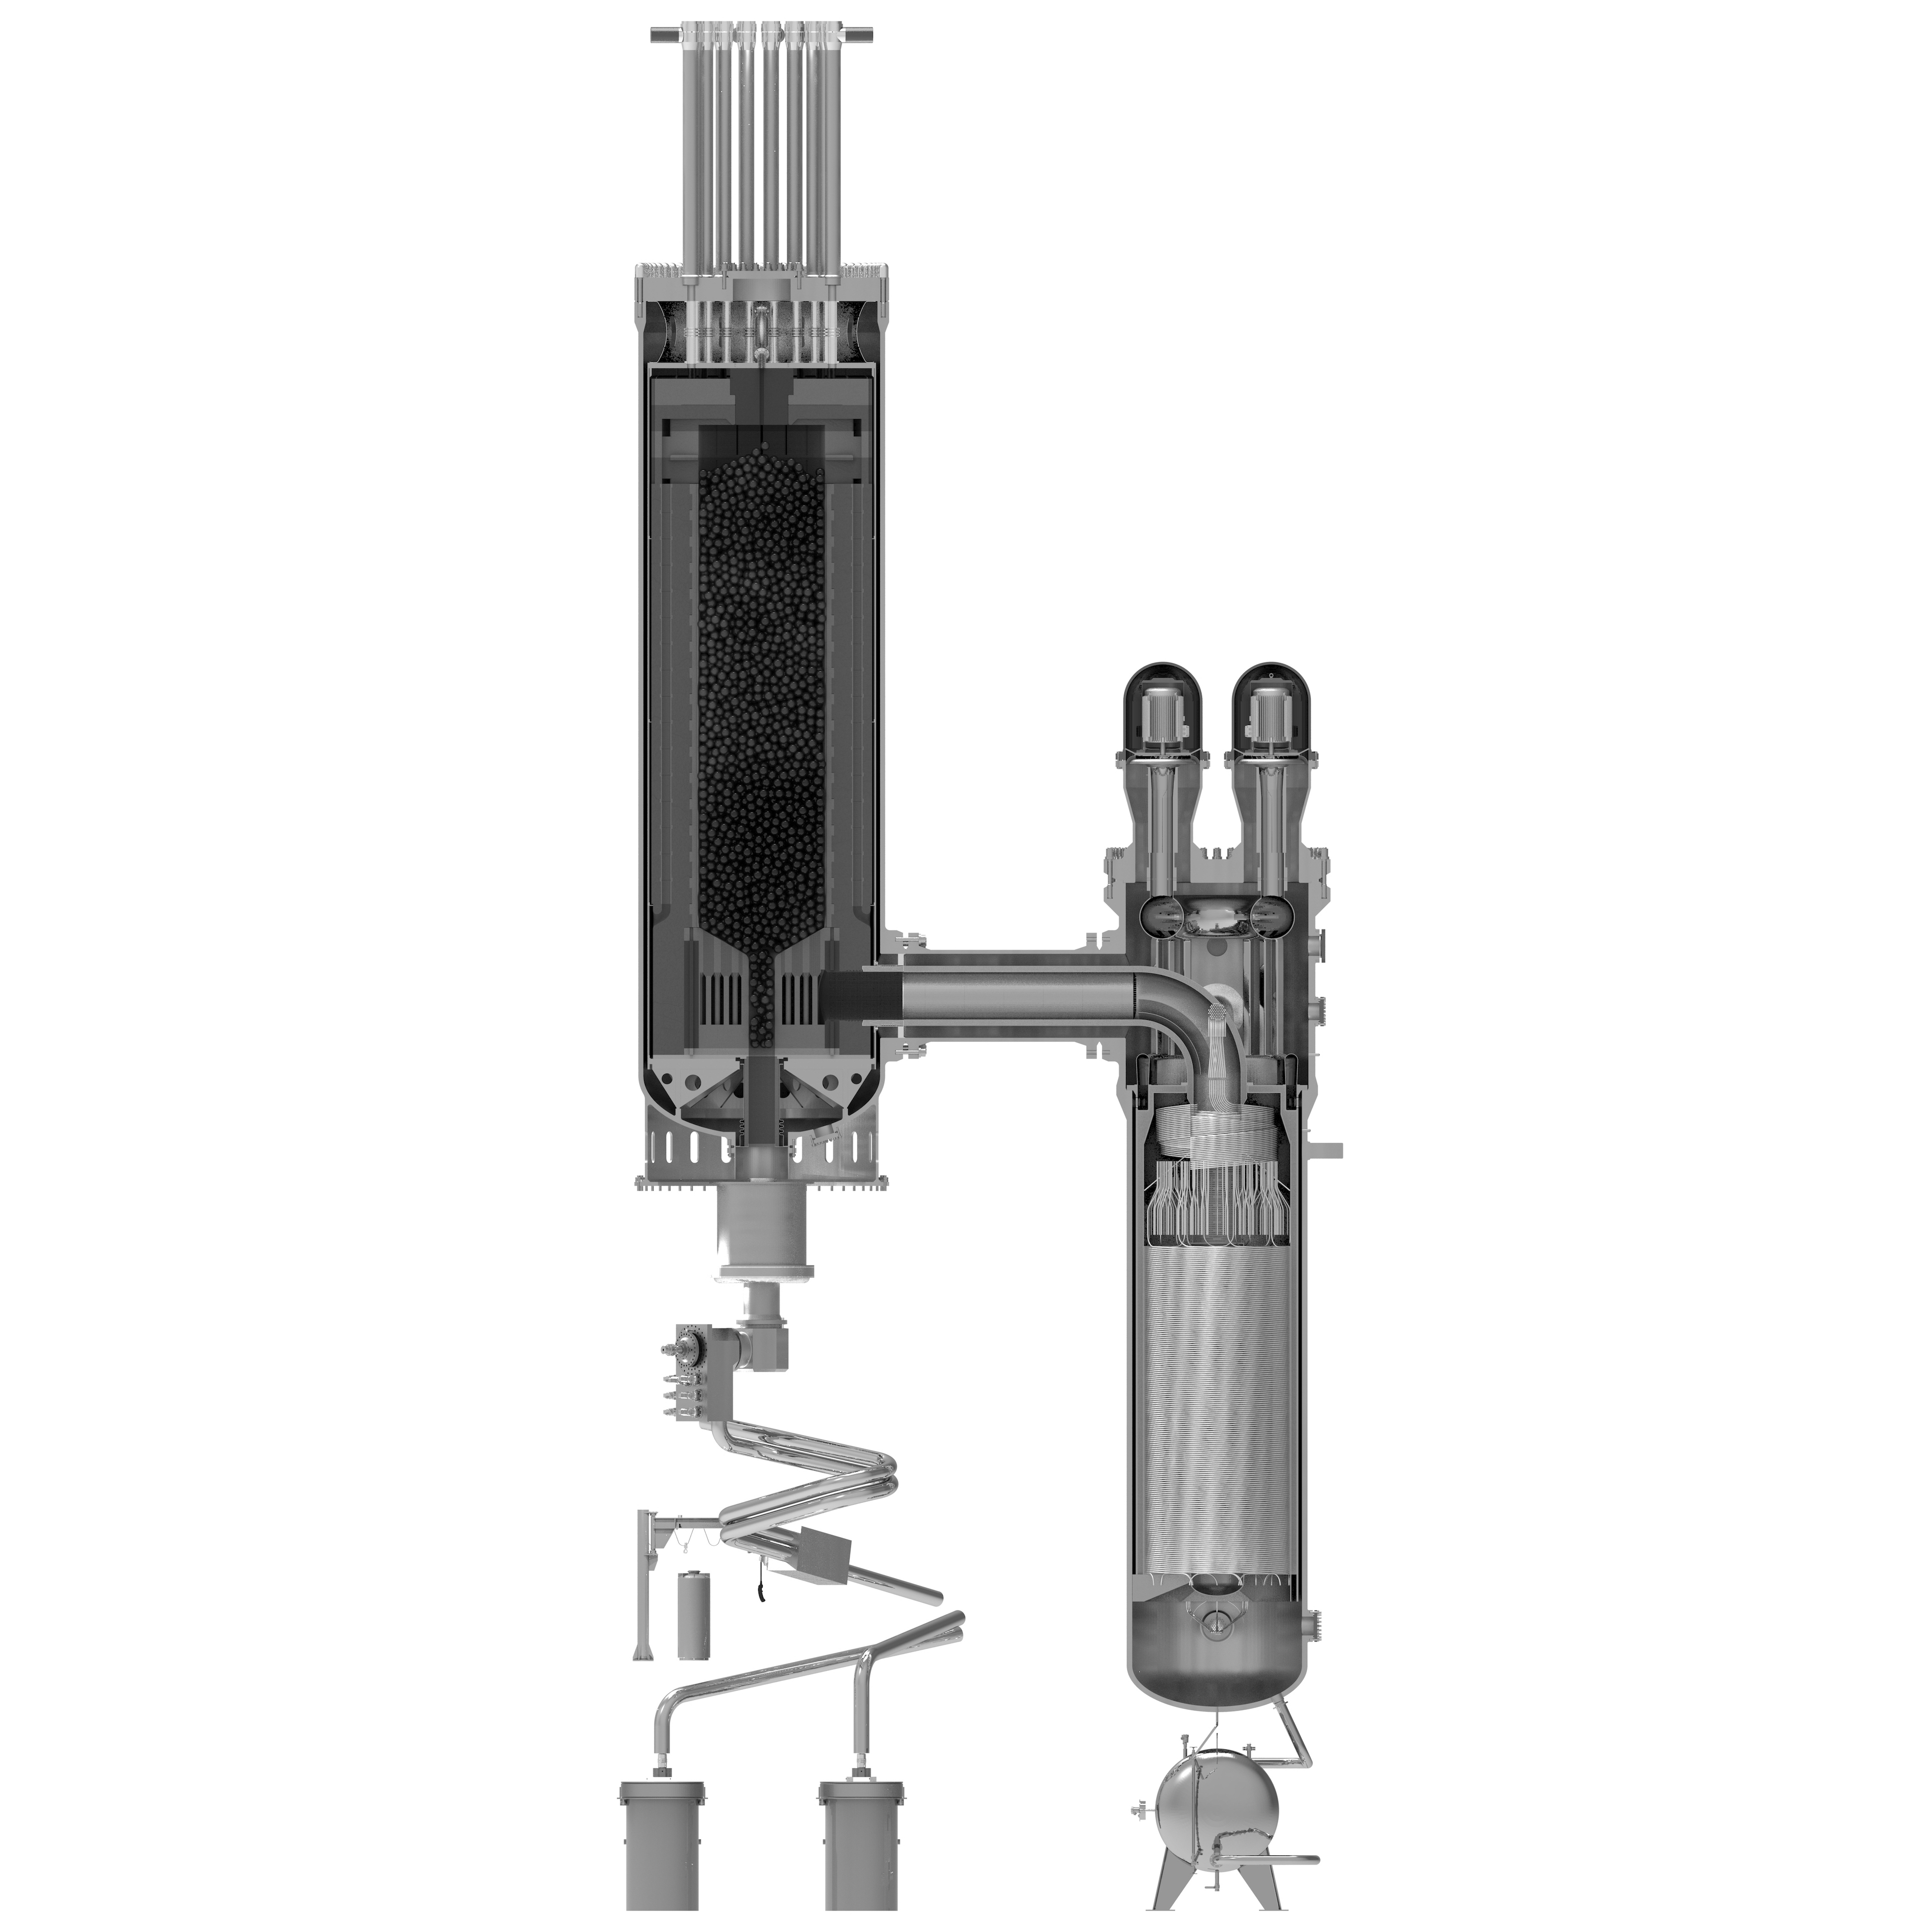
\includegraphics[scale=0.09]{images/reactor_design/xe-100-reactor-slice.jpg}
    \caption{X-Energy Xe-100 Rendition \cite{xe_reactor}}
    \label{fig:xe_design}
\end{figure}

Unlike the \gls{mmr}'s annular fuel elements, the \gls{xe} pebbles are composed of a graphite matrix that contains the \gls{triso} fuel particles. These \gls{triso} particles are very similar to those in the \gls{mmr}, as shown in Figure \ref{fig:xe_fuel}.

\begin{figure}[!htpb]
    \centering
    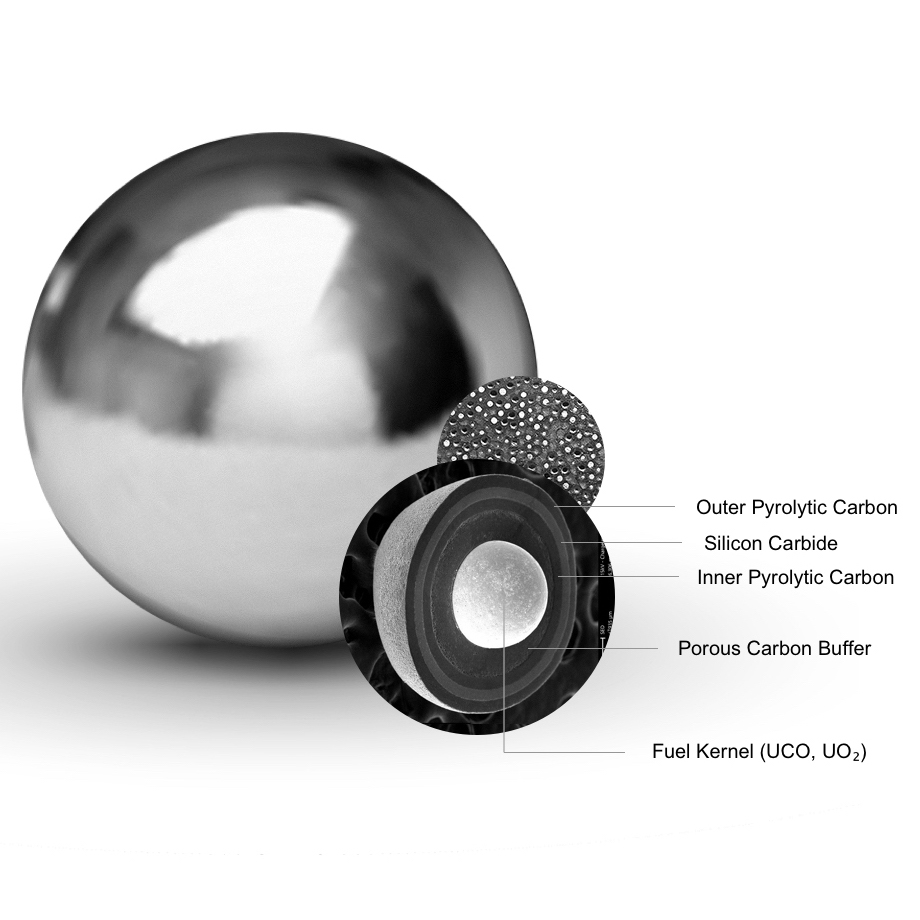
\includegraphics[scale=0.28]{images/reactor_design/graphic-triso-x-pebble.jpg}
    \caption{X-Energy Xe-100 Fuel Pebble \cite{xe_fuel}}
    \label{fig:xe_fuel}
\end{figure}


We have modified the fuel composition of Richter's \gls{xe}-like reactor model to accept \gls{leup} fuel. The \gls{leup} fuel is assumed to have the same burnup and power level as the \gls{haleu} fuel. This assumption is not necessarily valid, and we will explore the implications of this assumption in future work. However, we expect that, due to the limited deployment of \gls{leup} fuel, the discrepancies will be well-understood. Figure \ref{fig:xe_core} shows the top-down view of the \gls{xe} core model, we will not display both the \gls{leup} and \gls{haleu} versions of the core as they are established by Richter \cite{richter_thesis_2022}.

\begin{figure}[!ht]
    \subfloat[Initial core \label{fig:xe_init_core}]{%
      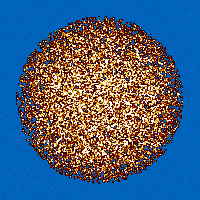
\includegraphics[width=0.49\textwidth]{images/reactor_design/htgr-mr-burn-200.inp_mesh1_bstep0.png}
   }
    \hfill
    \subfloat[Final core \label{fig:xe_final_core}]{%
      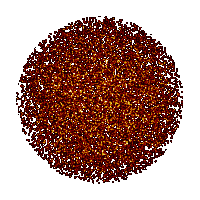
\includegraphics[width=0.49\textwidth]{images/reactor_design/htgr-mr-burn-200.inp_mesh1_bstep6.png}
   }
    \caption{Top-down view of the X-Energy Xe-100 core model.}
    \label{fig:xe_core}
  \end{figure}

Comparing Figures \ref{fig:xe_init_core} and \ref{fig:xe_final_core}, we can see visual differences in the shading of the pebbles. The pebbles are shaded based on the burnup of the fuel, with darker pebbles indicating higher burnup. The pebbles are inserted into the core at the top and gravity pulls them down through the core. After a brief holding time outside the core, the pebbles are reinserted at the top of the core. This process is repeated until the pebbles reach their targeted number of passes, at which point they are removed from the core and stored.

\subsection{AP1000 Reactor}
\label{sec:ap}

As of this writing, the AP1000 is operational in the \gls{usa} and China, and there are plans to deploy the reactor in the \gls{uk} and India. The Westinghouse AP1000 is a \gls{pwr} that uses UO$_2$ fuel. The reactor has a thermal output of 1000 MW and a cycle length of 18 years. The fuel is enriched to 5\% $^{235}$U and has a discharge burnup of 65 GWd/MTU. The reactor has a lifetime of 60 years. The reactor in this work is an approximation based on publicly available data and is not based on confidential or proprietary information. As this work does not anticipate \gls{leup} being used in the AP1000, there is no such neutronics model of the reactor and we have adapted the generic \cycamore reactor archetype to represent the AP1000 in the same way we represent the existing \gls{lwr} fleet.


